\section{Edge-preserving smoothing: bilateral and Kuwahara}

\textbf{Data.} The clean ground truth \code{q4.png} ($512\times512$) has a
200-level rectangle and a 20-level disc on a 60-level background, plus a
horizontal ramp from 66 to 103 that overlaps the disc. Its edges therefore range
from 140 levels (rectangle) down to 40 levels (disc against background). The
noisy input adds zero-mean Gaussian noise with $\sigma=20$ (seed 2026), which
gives 22.265 dB.

\subsection{Implementation and matched strength}

\textbf{Bilateral filter} \cite{tomasi} (\code{src/problem\_4/bilateral.py}):
\begin{equation}
g(\mathbf p)=\frac{\sum_{\mathbf q\in\Omega}w(\mathbf p,\mathbf q)f(\mathbf q)}{\sum_{\mathbf q\in\Omega}w(\mathbf p,\mathbf q)},\qquad
w(\mathbf p,\mathbf q)=\exp\!\Big(-\frac{\|\mathbf p-\mathbf q\|^2}{2\sigma_s^2}\Big)\exp\!\Big(-\frac{(f(\mathbf p)-f(\mathbf q))^2}{2\sigma_r^2}\Big),
\end{equation}
over a square window $\Omega$ of radius $r$ with reflected borders. Dividing by
the sum of the weights is the normalisation, so a flat region is left unchanged.
The code loops over the $(2r+1)^2$ window offsets, and each step is one array
operation over the whole image.

\textbf{Classical Kuwahara filter} \cite{kuwahara}
(\code{src/problem\_4/kuwahara.py}): for a window of size $N=2a+1$, I form the
four $(a+1)\times(a+1)$ sub-windows that share the centre row and column, and
output the mean of the one with the smallest variance. The sub-window sums of $f$
and $f^2$ come from two integral images, so the cost per pixel does not depend on
$N$.

\paragraph{(a) Matched smoothing strength.} The two filters have different
parameters, so ``the same amount of smoothing'' has to be defined first. I call
the filters matched when they
\begin{enumerate}
\item use the same footprint: the bilateral window radius equals the Kuwahara
half-width $a$, with $\sigma_s=a/2$ so that the window spans $\pm2\sigma_s$; and
\item reduce noise by the same amount where there is no edge: on a flat field
($256\times256$, value 128, the same $\sigma=20$, seed 11) the variance ratio
$\operatorname{var}(\text{output})/\operatorname{var}(\text{input})$ is the same.
\end{enumerate}
The first condition gives both filters the same neighbourhood to work with. The
second fixes the smoothing in flat regions, which is what ``strength'' means when
there is nothing to preserve. With both fixed, any difference at an edge can only
come from how each filter decides which neighbours to trust. That leaves
$\sigma_r$ as the only free parameter, and I find it by bisection on the variance
ratio.

\begin{table}[H]
\centering
\begin{tabular}{rrrrrr}
\toprule
$N$ & Kuwahara variance ratio & $\sigma_s$ & $\sigma_r$ & bilateral variance ratio & $1/(a+1)^2$\\
\midrule
5 & 0.12859 & 1.00 & 54.191 & 0.12859 & 0.11111\\
7 & 0.06906 & 1.50 & 51.918 & 0.06906 & 0.06250\\
11 & 0.02956 & 2.50 & 57.862 & 0.02956 & 0.02778\\
\bottomrule
\end{tabular}
\caption{Matched parameters (\code{matching.txt}). The matched $\sigma_r$ comes
out at 2.6 to 2.9 times the noise standard deviation.}
\label{tab:match}
\end{table}

The Kuwahara variance ratio is a bit above $1/(a+1)^2$, the variance ratio of a
single sub-window mean. The sub-windows share pixels, and which one gets chosen
depends on the same noise as its mean, so the selected mean is not an
independent average.

\paragraph{(b) Evaluation.}

\begin{table}[H]
\centering
\begin{tabular}{lrrr}
\toprule
Method & PSNR (dB) & SSIM & edge-band RMSE\\
\midrule
noisy input & 22.265 & 0.1674 & 19.506\\
Kuwahara $5\times5$ & 31.031 & 0.6069 & 8.114\\
bilateral $\sigma_s=1$, $\sigma_r=54.2$ & 30.941 & 0.5935 & 8.693\\
Kuwahara $7\times7$ & 33.558 & 0.7497 & 7.220\\
bilateral $\sigma_s=1.5$, $\sigma_r=51.9$ & 33.416 & 0.7384 & 7.823\\
Kuwahara $11\times11$ & 36.662 & 0.8788 & 7.294\\
bilateral $\sigma_s=2.5$, $\sigma_r=57.9$ & 36.139 & 0.8727 & 8.749\\
\bottomrule
\end{tabular}
\caption{Matched pairs against the clean image. Outputs are clipped to
$[0,255]$, data range 255. SSIM is my NumPy implementation of \cite{wang} with a
$7\times7$ uniform window, $K_1=0.01$, $K_2=0.03$ (checked against scikit-image
in the unit tests). The edge band is every pixel within 3 pixels of a
ground-truth jump larger than 5 levels; RMSE in 8-bit levels.}
\label{tab:edge-pres}
\end{table}

At every matched size Kuwahara is slightly ahead in PSNR (0.09 to 0.52 dB) and
SSIM, and clearly ahead near edges: its edge-band RMSE is 7.2 to 8.1 against 7.8
to 8.7. Since flat-region smoothing is equal by construction, the difference
comes from the edges, and the crops in Fig.~\ref{fig:edge-pres} show where. At
the 140-level rectangle edge both filters keep a sharp boundary. At the 40-level
disc edge the bilateral filter has a problem: with $\sigma_r=51.9$ a jump of 40
levels gets range weight $e^{-40^2/(2\cdot51.9^2)}=0.74$, almost as much as a
neighbour on the same side, so it averages across the edge and leaves it soft.
Kuwahara does not compare intensities pixel by pixel. It picks a whole
sub-window, usually one that lies on one side of the edge, so the boundary stays
sharp even at this contrast. With a step of 40 and noise of 20, the extra variance
of a sub-window that straddles the edge (about $p(1-p)\cdot40^2\le400$) is no
larger than the noise variance, so the choice is not always right, which is why
the boundary is slightly ragged. Kuwahara's own artifact shows in the flat areas:
a patchwork of small flat blocks instead of the bilateral filter's smooth
leftover texture.

\begin{figure}[H]
\centering
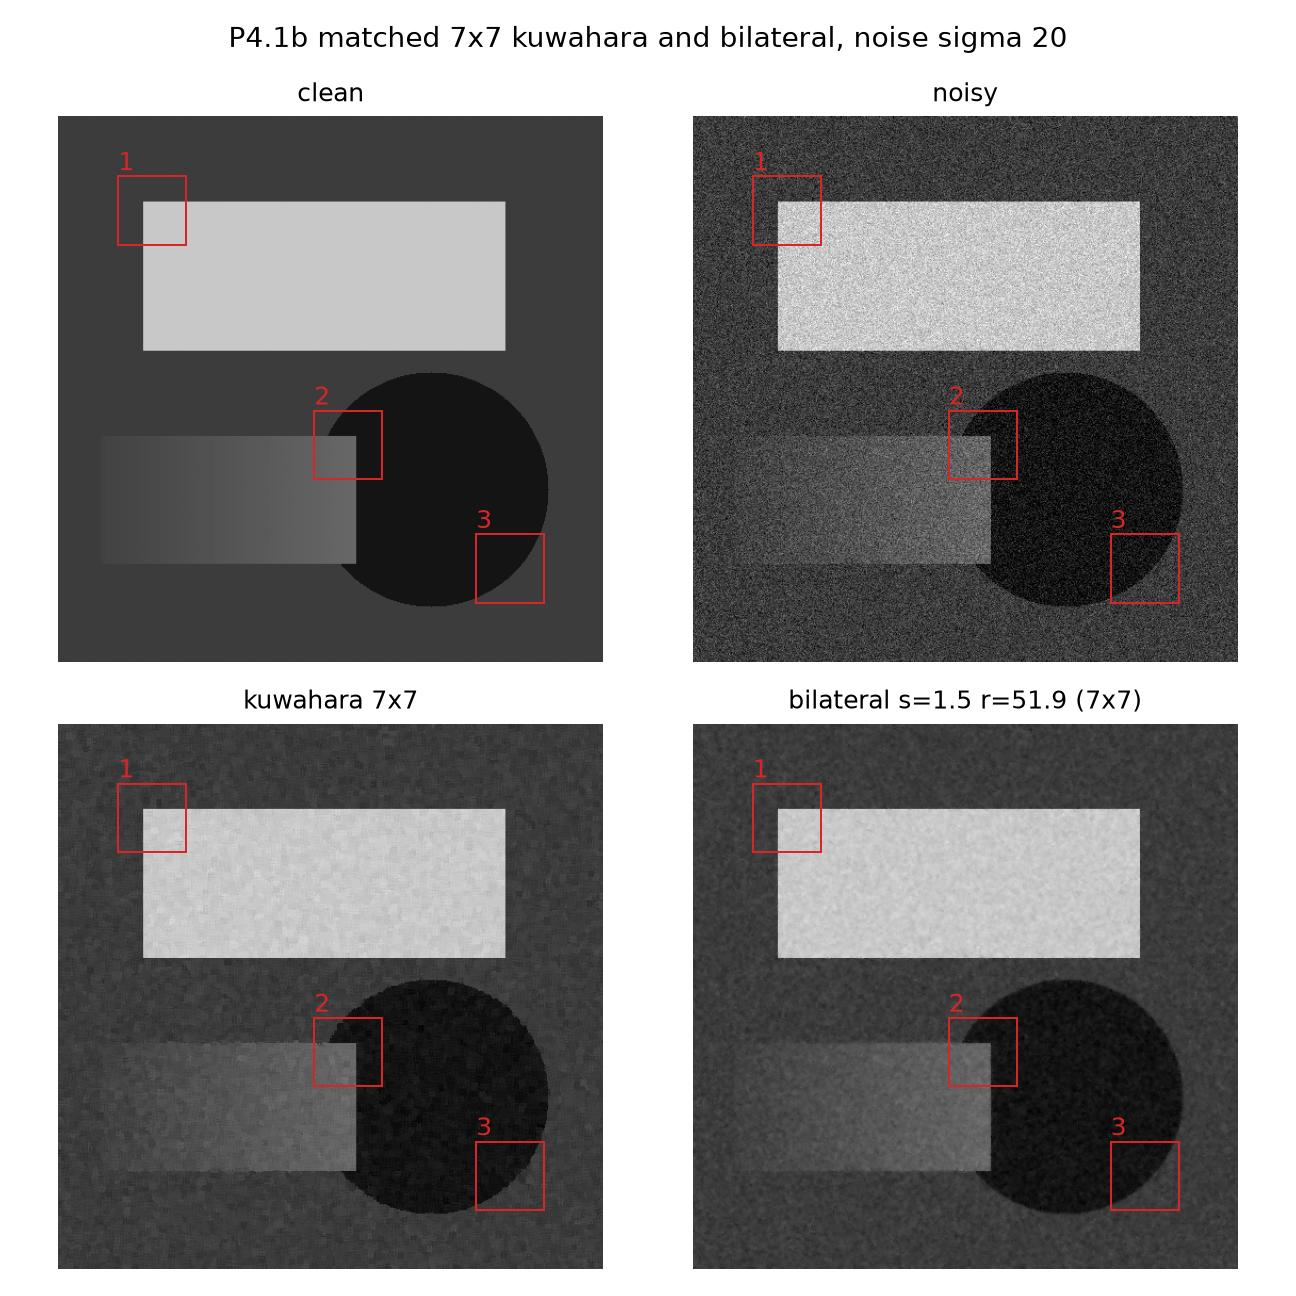
\includegraphics[width=0.92\linewidth]{problem_4/edge_preservation_comparison.png}
\caption{Matched $7\times7$ pair. Rows 2 to 4 are the $64\times64$ crops boxed in
red: the rectangle corner (contrast 140), the ramp crossing the disc, and the
disc edge (contrast 40).}
\label{fig:edge-pres}
\end{figure}

\subsection{Kuwahara blockiness and complexity}

\paragraph{(a) Why the hard argmin makes blocks.} In a flat noisy region, each of
the four sub-window means changes slowly as the window slides, because it is a
moving average. Which of the four has the smallest variance is a discrete choice,
though, and it can flip from one pixel to the next. When it flips, the output
jumps from one sub-window mean to another, a step that is not in the input.
Neighbouring windows share most of their pixels, so the same sub-window tends to
win over a whole patch. The output becomes patches of nearly constant value
separated by small steps, the painterly blocks, and their size grows with the
sub-window. This is not blur, because the chosen sub-window lies on one side of an
edge and never averages across it. It is not ringing either: the output is always
the plain mean of input samples, a weighted average with non-negative weights, so
by the argument in 2.2(b) it stays inside the local range of the input and cannot
overshoot.

\paragraph{(b) Soft Kuwahara.} My modification replaces the argmin with softmax
weights on the negative variances,
\begin{equation}
g=\frac{\sum_{k=1}^4 w_k m_k}{\sum_k w_k},\qquad
w_k=\exp\!\Big(-\frac{s_k^2-\min_j s_j^2}{T}\Big),\qquad T=\sigma^2=400,
\end{equation}
with $m_k$ and $s_k^2$ the sub-window means and variances. Subtracting the
minimum only guards against underflow and cancels in the ratio. The output is now
a continuous function of the variances, so it cannot jump when two of them swap
order. Near a strong edge, a sub-window that straddles it has its variance raised
by about $p(1-p)\Delta I^2$ (4900 for half of a 140-level step), which gives it
weight $e^{-12}$, so it is still left out, as in the classical filter. With
$T=\sigma^2$, two sub-windows whose variances differ by about the noise variance
are blended instead of chosen between. I measure blockiness away from the true
edges (242792 pixels at least 4 pixels from any jump) by the total variation
$\overline{|\partial_xg|+|\partial_yg|}$ and by the 99th percentile of
$|\nabla g|$. Both are tiny on the clean image (0.017 and 1.000).

\begin{table}[H]
\centering
\begin{tabular}{rlrrrrr}
\toprule
$N$ & method & TV & p99 $|\nabla g|$ & PSNR (dB) & SSIM & edge RMSE\\
\midrule
11 & classical & 4.436 & 12.556 & 36.662 & 0.8788 & 7.294\\
11 & soft & 1.751 & 3.477 & 39.866 & 0.9638 & 6.870\\
15 & classical & 2.997 & 9.240 & 38.304 & 0.9270 & 7.679\\
15 & soft & 1.141 & 2.367 & 40.401 & 0.9764 & 7.794\\
\bottomrule
\end{tabular}
\caption{Classical and soft Kuwahara at identical window sizes
(\code{blockiness.txt}). TV and gradients in grey levels per pixel.}
\label{tab:block}
\end{table}

The soft version cuts the total variation by 61\,\% at $N=11$ and 62\,\% at
$N=15$, and the 99th-percentile gradient (the size of the larger block steps) by
72\,\% and 74\,\%. PSNR rises by 3.2 and 2.1 dB. Edge RMSE improves at $N=11$ and
gets slightly worse at $N=15$ (7.79 against 7.68). At the low-contrast disc edge
the variance of a straddling sub-window only rises by about 400, so it keeps
weight $e^{-1}$ and the edge gets mixed a little. Fig.~\ref{fig:block} shows the
ramp, where the classical filter turns a smooth gradient into flat steps and the
soft filter keeps it smooth, and the rectangle corner, which both keep sharp.

\begin{figure}[H]
\centering
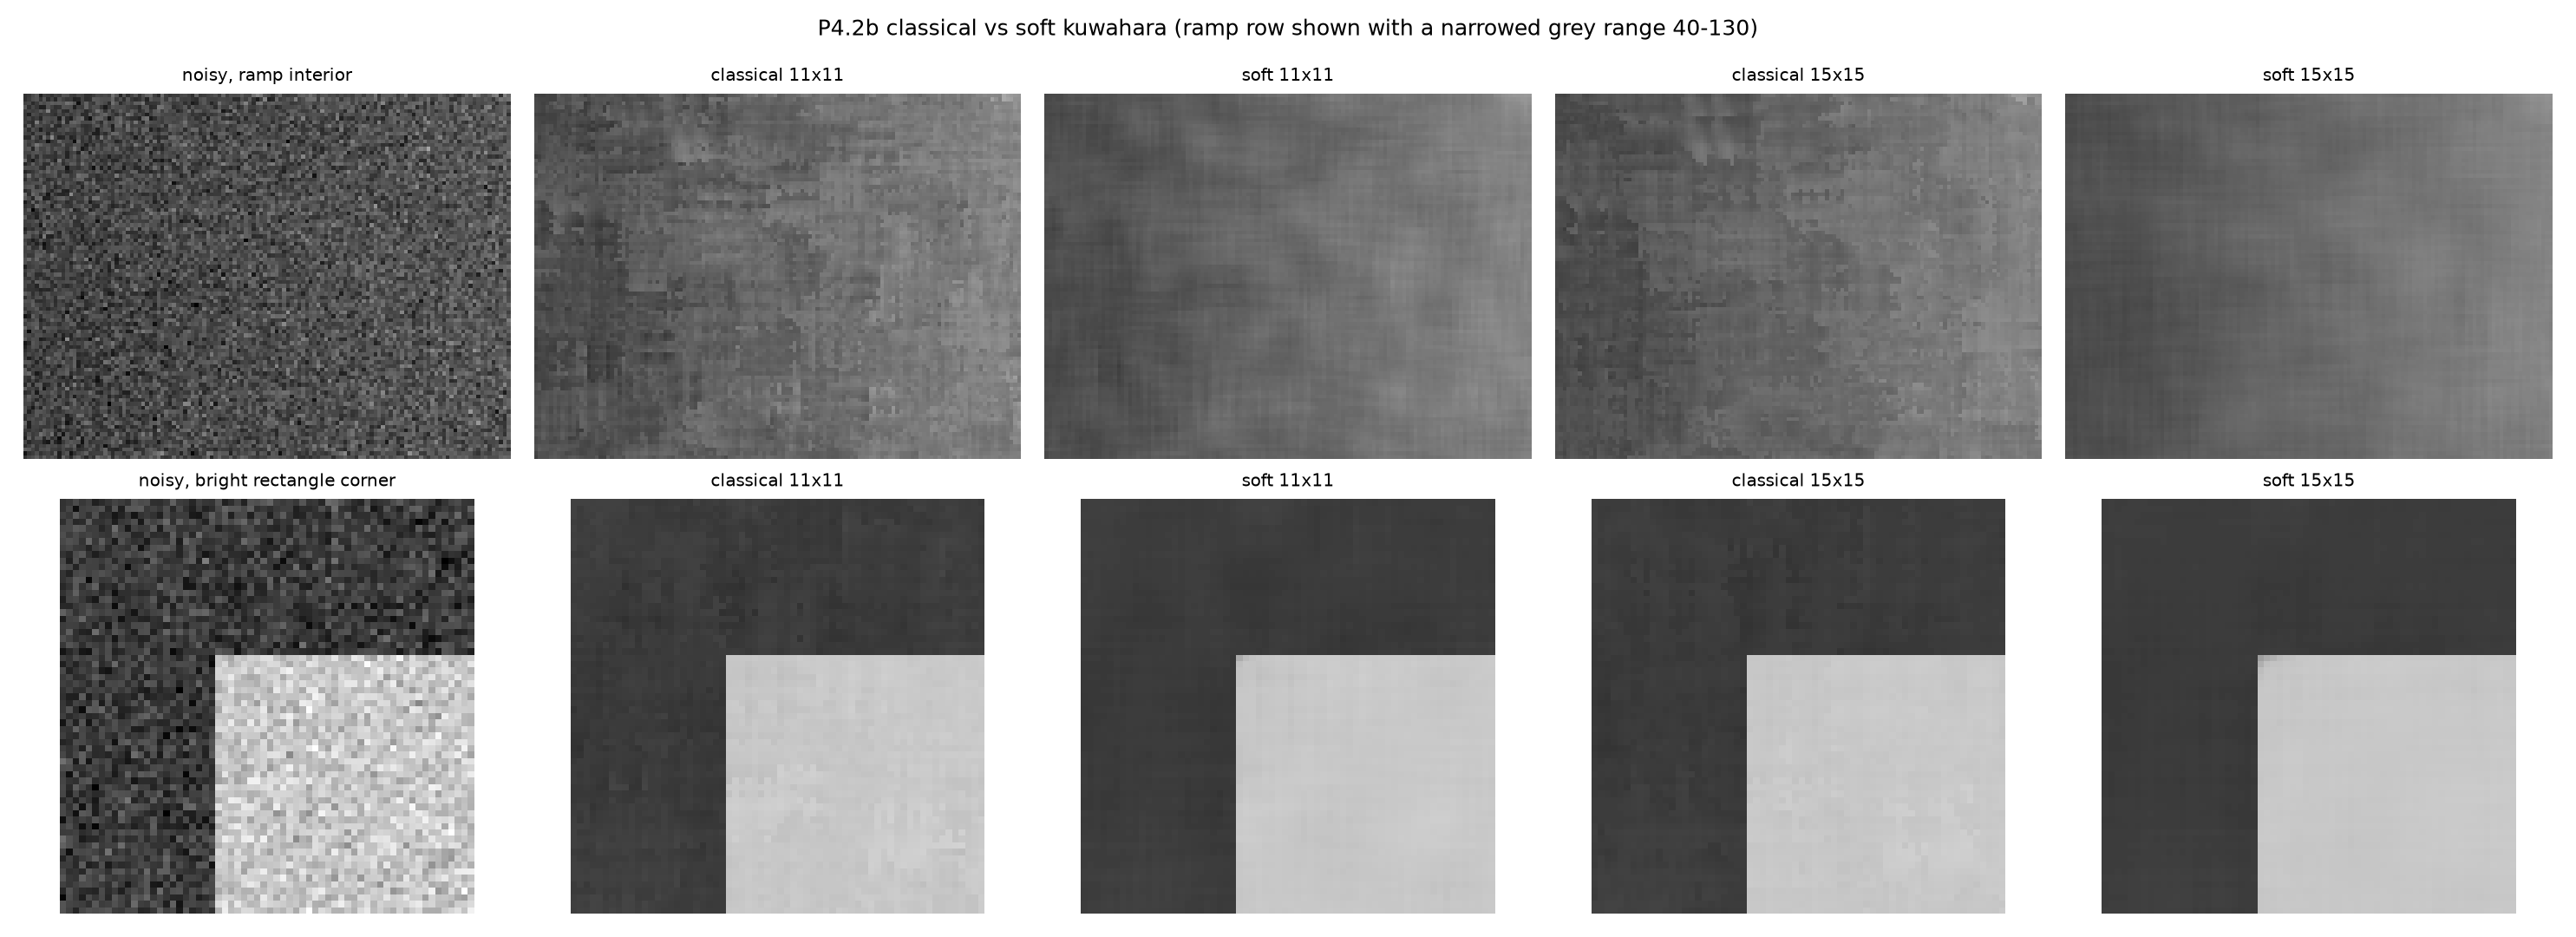
\includegraphics[width=\linewidth]{problem_4/blockiness.png}
\caption{Classical and soft Kuwahara at $11\times11$ and $15\times15$. Top: the
inside of the ramp, shown with a narrowed grey range of 40 to 130. Bottom: the
rectangle corner.}
\label{fig:block}
\end{figure}

\paragraph{(c) Operations per pixel.} I count additions and subtractions
(including comparisons), multiplications and divisions, and exponentials for one
output pixel.
\begin{itemize}
\item \emph{Kuwahara with integral images:} building the two integral images
costs 1 square and 4 additions. Each of the four sub-windows costs 6 additions or
subtractions for the two box sums, 1 subtraction for the variance and 3
multiplications or divisions. The argmin is 3 comparisons. Total: 35, 13, 0, the
same for every $N$.
\item \emph{Kuwahara with direct sums:} $4\cdot2((a+1)^2-1)+7$ additions and
$4(a+1)^2+12$ multiplications, i.e.\ $O(N^2)$.
\item \emph{Soft Kuwahara:} the integral-image count plus 4 subtractions, 4
divisions by $T$ and 4 exponentials for the weights, and 6 additions, 4
multiplications and 1 division for the weighted mean. Total: 45, 22, 4.
\item \emph{Bilateral:} per window tap, 1 subtraction, 1 square, 1 scaling, 1
exponential, 1 multiplication by the spatial weight, 1 by the value and 2
additions, plus one division per pixel: $3N^2$, $4N^2+1$, $N^2$.
\end{itemize}

\begin{table}[H]
\centering
\begin{tabular}{rlrrrr}
\toprule
$N$ & filter & add/sub/cmp & mult/div & exp & runtime (s)\\
\midrule
5 & Kuwahara (integral) & 35 & 13 & 0 & 0.0148\\
5 & soft Kuwahara & 45 & 22 & 4 & 0.0151\\
5 & bilateral & 75 & 101 & 25 & 0.0355\\
7 & Kuwahara (integral) & 35 & 13 & 0 & 0.0143\\
7 & Kuwahara (direct) & 127 & 76 & 0 & not timed\\
7 & bilateral & 147 & 197 & 49 & 0.0644\\
11 & Kuwahara (integral) & 35 & 13 & 0 & 0.0152\\
11 & bilateral & 363 & 485 & 121 & 0.1595\\
15 & Kuwahara (integral) & 35 & 13 & 0 & 0.0135\\
15 & soft Kuwahara & 45 & 22 & 4 & 0.0144\\
15 & bilateral & 675 & 901 & 225 & 0.3037\\
\bottomrule
\end{tabular}
\caption{Operation counts per pixel and measured run times on the $512\times512$
noisy image, median of 3 runs (all rows in \code{complexity.txt}). The
$15\times15$ bilateral uses $\sigma_s=3.5$, $\sigma_r=40$, since I did not
compute a matched pair at that size.}
\label{tab:complexity}
\end{table}

The bilateral filter is by far the most expensive per pixel. It needs an
exponential for every tap, because the range weight depends on the intensity
difference and cannot be computed in advance, and its work grows with the window
area ($N^2$ exponentials). Kuwahara only needs box statistics, which integral
images give in constant time, so its run time stays around 0.014 s from
$5\times5$ to $15\times15$ while the bilateral filter grows from 0.036 to
0.304 s. The four exponentials of the soft version add at most about 0.001 s.

\subsection{Breakdown of the bilateral filter}

\paragraph{(a, b) Experiment.} Each test image is $256\times128$, split into
$I_1=100$ and $I_2=150$ ($|\Delta I|=50$), with fresh Gaussian noise for every
NCR $=\sigma/|\Delta I|$ from 0.05 to 1.5 and 8 noise images per value (seed
$1000\cdot\text{index}+k$). The bilateral filter uses $\sigma_s=2$, radius 6,
and $\sigma_r=2\sigma$, a typical setting, since the range scale has to exceed
the noise for the filter to smooth at all. My edge-preservation metric is the
largest jump between neighbouring columns of the output profile, averaged over
rows and over the eight images, divided by $|\Delta I|$: 1 means the step is still
one pixel wide. A plain spatial Gaussian with the same $\sigma_s$ keeps 0.1997. I
define $\text{NCR}^*$ as the NCR where the curve falls to halfway between these
two levels, i.e.\ to 0.5998.

\begin{figure}[H]
\centering
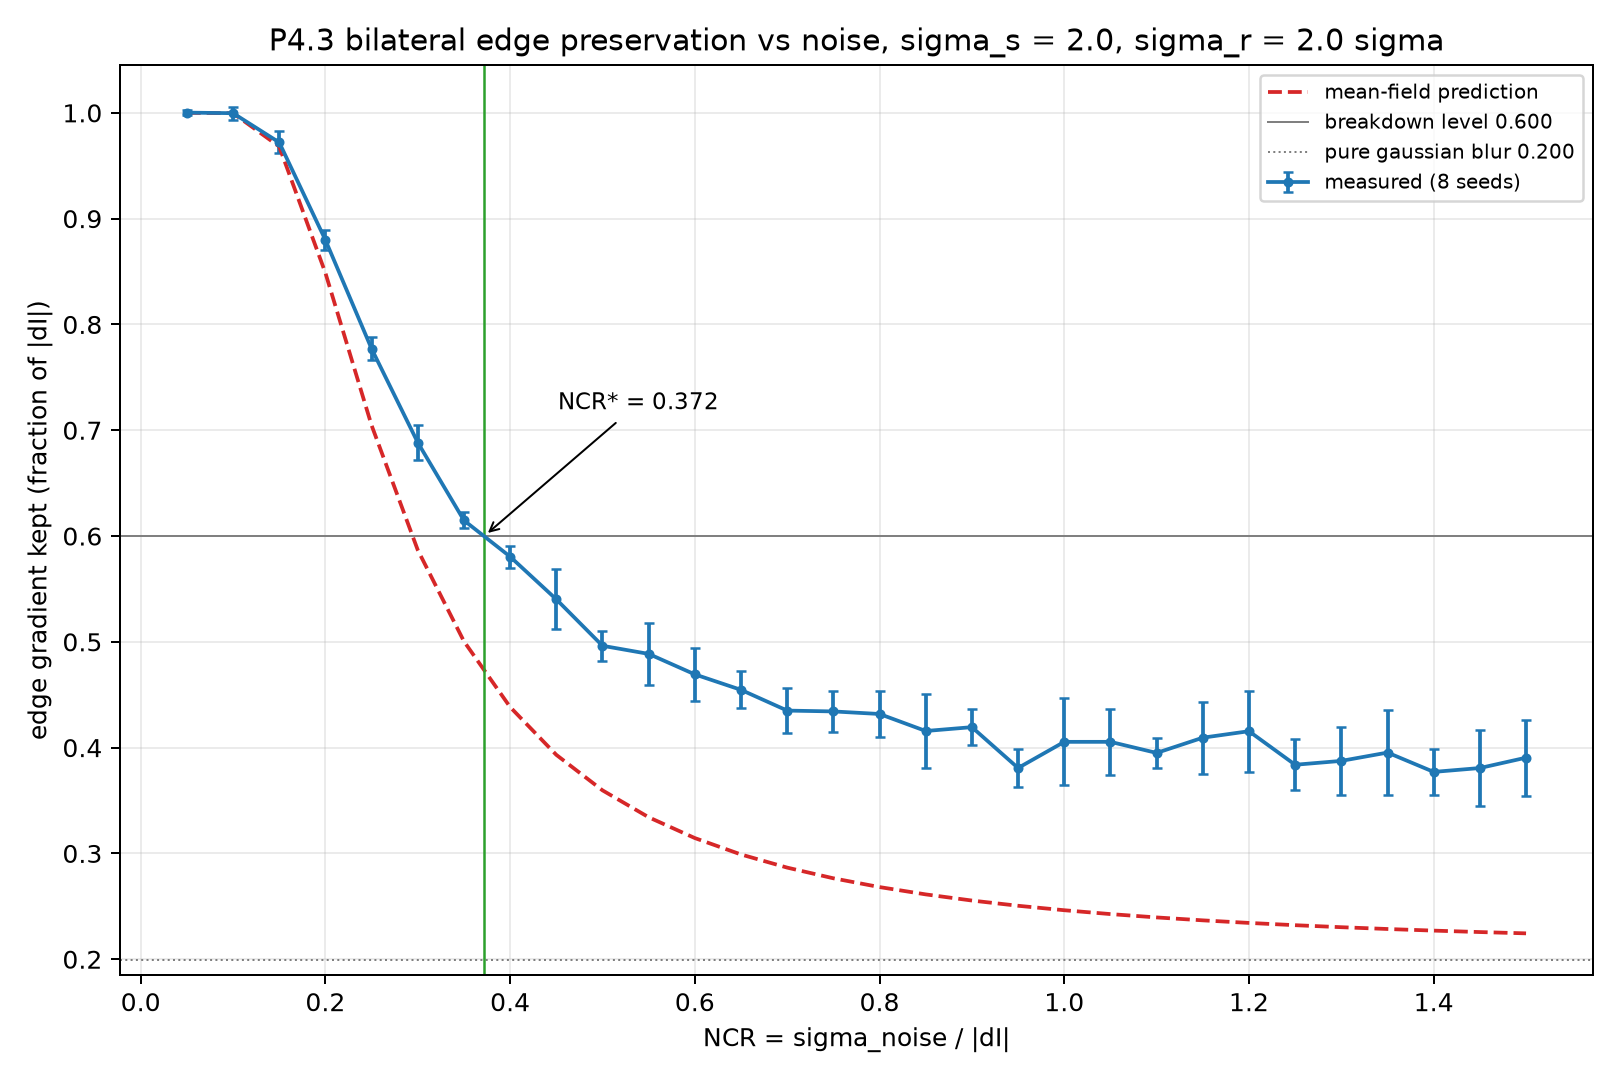
\includegraphics[width=0.75\linewidth]{problem_4/ncr_breakdown.png}
\caption{Fraction of the edge gradient kept against NCR (mean and spread over 8
noise images), with the mean-field prediction and the measured $\text{NCR}^*$.}
\label{fig:ncr}
\end{figure}

\begin{table}[H]
\centering
\begin{tabular}{rrrrrr}
\toprule
NCR & gradient kept & spread & edge RMSE & mean-field & $\rho$\\
\midrule
0.10 & 0.9997 & 0.0061 & 1.484 & 0.9997 & 0.0002\\
0.20 & 0.8799 & 0.0093 & 4.815 & 0.8487 & 0.1245\\
0.30 & 0.6884 & 0.0166 & 8.375 & 0.5868 & 0.3962\\
0.35 & 0.6148 & 0.0077 & 9.719 & 0.5005 & 0.5065\\
0.40 & 0.5805 & 0.0105 & 10.583 & 0.4384 & 0.5940\\
0.50 & 0.4963 & 0.0141 & 12.340 & 0.3596 & 0.7165\\
1.00 & 0.4055 & 0.0412 & 18.102 & 0.2463 & 0.9200\\
1.50 & 0.3905 & 0.0358 & 23.621 & 0.2244 & 0.9636\\
\bottomrule
\end{tabular}
\caption{Selected rows of \code{ncr\_breakdown.txt}. Edge RMSE in grey levels.}
\label{tab:ncr}
\end{table}

The measured curve crosses that level at $\textbf{NCR}^*\mathbf{=0.372}$. Below
about 0.15 the step survives intact, and by 0.5 half of its gradient is gone
(examples in \code{ncr\_examples.png}).

\paragraph{(c) Why it breaks down.} The range kernel
$w_r(\Delta I)=e^{-\Delta I^2/2\sigma_r^2}$ is supposed to give small weight to
neighbours across the edge and large weight to neighbours on the same side. With
noise, the difference the filter actually sees is $d=f(\mathbf p)-f(\mathbf q)$,
which is distributed as $\mathcal N(0,2\sigma^2)$ on the same side and
$\mathcal N(\Delta I,2\sigma^2)$ across the edge. Averaging the Gaussian kernel
over a Gaussian difference gives
\begin{equation}
\operatorname{E}[w_r]=\frac{\sigma_r}{\sqrt{\sigma_r^2+2\sigma^2}}\cdot
\begin{cases}1&\text{same side}\\ e^{-\Delta I^2/2(\sigma_r^2+2\sigma^2)}&\text{across}\end{cases},
\qquad
\rho=\exp\!\Big(-\frac{\Delta I^2}{2(\sigma_r^2+2\sigma^2)}\Big)=\exp\!\Big(-\frac{1}{2\,\text{NCR}^2(k^2+2)}\Big),
\end{equation}
with $\sigma_r=k\sigma$ and $\rho$ the ratio of the expected cross-edge weight to
the same-side weight. The noise widens the effective range kernel from $\sigma_r$
to $\sqrt{\sigma_r^2+2\sigma^2}$. Once that width is comparable to the step,
$\rho$ approaches 1 and neighbours across the edge are trusted almost as much as
those on the same side, so the filter turns into a spatial blur. $\rho$ passes
$1/2$ at $\text{NCR}=1/\sqrt{2\ln2\,(k^2+2)}=0.347$ for $k=2$, close to the
measured 0.372. The change is gradual because $\rho$ rises smoothly, from 0.12 at
NCR 0.2 to 0.72 at 0.5.

Plugging the expected weights in place of the random ones (the ``mean-field''
column, which also gives the centre pixel its exact weight of 1) predicts the
onset fairly well, crossing the midpoint at 0.2945. It does not predict the
high-noise level: the measured curve levels off at 0.395 instead of falling
towards 0.2. The model treats the weights as independent of the values, but they
are not: neighbours whose noisy values happen to be close to the centre pixel's
value get the largest weights, which pulls the output towards the centre pixel
and keeps part of the step. Because $\sigma_r$ grows with $\sigma$, this does not
fade as the noise grows. Measured against that plateau instead of the Gaussian
level, the halfway point is at NCR 0.295.
